\begin{example}
  [Example with Two Paths Iterating Alternatively and Nested Loop with Related Counters]
  \label{ex:relatedNestedWhileOdd}
  { \small
  \begin{figure}
  \centering
  \begin{subfigure}{.4\textwidth}
    \begin{centering}
    {\small
    $
    \begin{array}{l}
      \kw{relatedNestedWhileOdd}(n, m) \triangleq \\
      \clabel{ \assign{i}{n} }^{0} ; \\
          \ewhile ~ \clabel{i > 0}^{1} ~ \edo ~ \\
          \qquad \Big(
            \eif(\clabel{i \% 2 = 0 }^{2},\\
            \qquad \clabel{\assign{k}{i - m}}^{3};\\
            \qquad \ewhile ~ \clabel{k > 0}^{4} ~ \edo ~
            \Big( \clabel{\assign{j}{j - 1}}^{5} \Big);\\
            \qquad \clabel{\assign{i}{k + m}}^{6};
            \clabel{\assign{i}{i - 1}}^{7}, \\
            \qquad \clabel{\assign{i}{i - 3}}^{8});
            \Big)
      \end{array}
    $
    }
    \caption{}
    \end{centering}
    \end{subfigure}
  \begin{subfigure}{.5\textwidth}
    \begin{centering}
  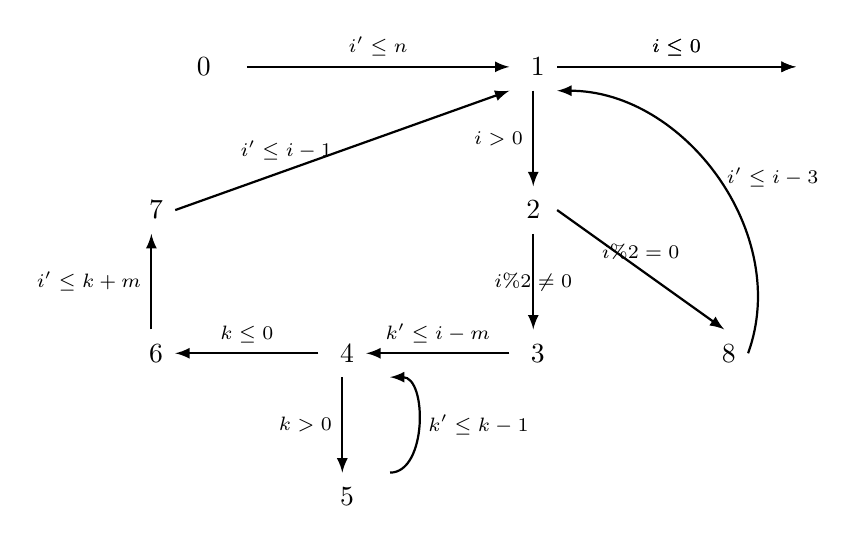
\begin{tikzpicture}[scale=\textwidth/20cm,samples=200]
  \draw[] (-7, 10) circle (0pt) node{{ $0$}};
  \draw[] (0, 10) circle (0pt) node{{ $1$}};
  \draw[] (0, 7) circle (0pt) node{\textbf{$2$}};
  \draw[] (0, 4) circle (0pt) node{{ $3$}};
  \draw[] (-4, 4) circle (0pt) node{{ $4$}};
  \draw[] (-8, 4) circle (0pt) node{{ $6$}};
  \draw[] (-4, 1) circle (0pt) node{{ $5$}};
  \draw[] (4, 4) circle (0pt) node{{ $8$}};
  \draw[] (-8, 7) circle (0pt) node{{ $7$}};
  % Counter Variables
  \draw[] (6, 10) circle (0pt) node {\textbf{$\lex$}};
  % \draw[] (6, 4) circle (0pt) node {{ $ex$}};
  %
  % Control Flow Edges:
  \draw[ thick, -latex] (-6, 10)    -- node [above] {\scriptsize $i' \leq n$}(-0.5, 10);
  \draw[ thick, -latex] (0, 9.5)    -- node [left] {\scriptsize $i > 0$} (0, 7.5) ;
  \draw[ thick, -latex] (0.5, 7)    -- node [above] {\scriptsize $ i \% 2 = 0 $}  (4, 4.5);
  \draw[ thick, -latex] (4.5, 4)    to  [out=70,in=0]   node [right] {\scriptsize $i' \leq i - 3$ }(0.5, 9.5);
  \draw[ thick, -latex]  (0, 6.5)   -- node  {\scriptsize $i \% 2 \neq 0$}  (0, 4.5) ;
  \draw[ thick, -latex]  (-0.5, 4)  -- node [above] {\scriptsize $k' \leq i - m$ }  (-3.5, 4) ;
  \draw[ thick, -latex]  (-4.5, 4)  -- node [above] {\scriptsize $k \leq 0$ }  (-7.5, 4);
  \draw[ thick, -latex] (0.5, 10)   -- node [above] {\scriptsize $i \leq 0$}  (5.5, 10);
  \draw[ thick, -latex] (-4, 3.5)   -- node [left] {\scriptsize $k > 0$}  (-4, 1.5);
  \draw[ thick, -latex] (-3, 1.5)   to  [out=0,in=0] node [right] {\scriptsize $k' \leq k- 1$}  (-3, 3.5);
  \draw[ thick, -latex] (0.5, 10)   -- node [above] {\scriptsize $i \leq 0$}  (5.5, 10);
  \draw[ thick, -latex] (-8, 4.5)   --  node [left] {\scriptsize $i' \leq k + m$ }(-8, 6.5);
  \draw[ thick, -latex] (-7.5, 7)  --  node [left] {\scriptsize $i' \leq i - 1$ }(-0.5, 9.5);
  % \draw[ thick, -latex] (6, 6.5)  -- node [right] {$\top$} (6, 4.5) ;
  \end{tikzpicture}
  \caption{}
    \end{centering}
    \end{subfigure}
  \caption{
  (a) The program of the two paths loop with a nested Loop in one path
    (b) The Abstract Execution Control Flow Graph}
      \label{fig:relatedNestedWhileOdd}
  \end{figure}
  }
  %
  \end{example}    
  \begin{enumerate}
    \item  \textbf{The Abstract Execution Control Flow Graph} is generated in Figure~\ref{fig:relatedNestedWhileOdd}(b).
    \item \textbf{Program Refinement}
    \\
    The loop free simple transition paths are computed as follows,
    \\ 
    $\tpath_0 = (0 \to 1)$
      \quad
      $\tpath_1 = (1 \to 2 \to 3 \to 4)$
      \quad
      $\tpath_2 = (4 \to 6 \to 7 \to 1)$
      \quad
      $\tpath_3 = (4 \to 5 \to 4)$
      \quad
      $\tpath_4 = (1 \to 2 \to 8 \to 1)$
      \quad
      $\tpath_5 = (1 \to \lex)$

  \textbf{Refined Program}:
    \[
    \tpath_0 ; \rpchoose{ 1: \rprepeat(\tpath_1; 4:\rprepeat(\tpath_3); \tpath_2; \tpath_4), 
    1: \rprepeat(\tpath_4; \tpath_1; 4:\rprepeat(\tpath_3); \tpath_2) }; \tpath_5
    \]
    Let $\rprog_1^1 = \rprepeat(\tpath_1; 4:\rprepeat(\tpath_3); \tpath_2; \tpath_4)$
    \\
    $\rprog_1^2 = \rprepeat(\tpath_4; \tpath_1; 4:\rprepeat(\tpath_3); \tpath_2) $
    %
    \item {Path Local Reachability-bound}:
    \\
    $\outinB(\rprog, \tpath_0) = 1$ \\
    $\outinB(\rprog, \tpath_4) = 1$ \\
    $\outinB(1: \rprog_1^1, \tpath_1) = \frac{m}{4}$ \\
    $\outinB(1: \rprog_1^1, \tpath_2) = \frac{m}{4}$ \\
    $\outinB(1: \rprog_1^1, \tpath_4) = \frac{m}{4}$ \\
    $\outinB(1: \rprog_1^2, \tpath_1) = \frac{m}{4}$ \\
    $\outinB(1: \rprog_1^2, \tpath_2) = \frac{m}{4}$ \\
    $\outinB(1: \rprog_1^2, \tpath_4) = \frac{m}{4}$ \\
    $\outinB(4: \rprepeat(\tpath_3), \tpath_3) = n - m$ 
    \\
    Loop Bounds:
    \\
    $BD(\tpath_0) = 1$
    \quad
    $BD(\tpath_5) = 1$
    \quad
    $BD(\rprepeat(\tpath_3)) = n - m $
    \quad
    $BD(\rprog_1^1) = \frac{m}{4} $
    \quad
    $BD(\rprog_1^2) = \frac{m}{4} $

    %
    \item Loop Reachability-bound:
    \\
    \highlight{
    $\lpchB(1: \rprog_1^1, \tpath_1) = \frac{n-m}{4}$ \quad
    $\lpchB(1: \rprog_1^1, \tpath_2) = \frac{m}{4}$ \quad 
    $\lpchB(1: \rprog_1^1, \tpath_4) = \frac{m}{4}$ \\
    \highlight{$\lpchB(1: \rprog_1^1, \tpath_3) = 1$} \quad 
    $\lpchB(1: \rprog_1^2, \tpath_1) = \frac{m}{4}$ \quad
    $\lpchB(1: \rprog_1^2, \tpath_2) = \frac{m}{4}$ \\
    $\lpchB(1: \rprog_1^2, \tpath_4) = \frac{m}{4}$ \quad 
    \highlight{$\lpchB(1: \rprog_1^2, \tpath_2) = 1$} \quad
    $\lpchB(5: \rprepeat(\tpath_2), \tpath_2) = n - m$ 
    }
    %
    %
    \item Path Global Reachability-bound:
    \\
    $\inoutB(\rprog, \tpath_0) = 1$ \quad
    $\inoutB(\rprog, \tpath_1) = \frac{m}{4}$ \quad
    $\inoutB(\rprog, \tpath_2) = \frac{m}{4}$ \\
    $\inoutB(\rprog, \tpath_3) = \frac{m}{4} \times 1$ \quad
    $\inoutB(\rprog, \tpath_4) = \frac{m}{4}$ \quad
    $\inoutB(\rprog, \tpath_5) = 1$
    %
    \item The Reachability-bound:
    \\
    $\psRB(0) = \psRB(\lex) = 1$ \quad
    $\psRB(1) = \frac{m}{2} + 1$ \quad
    $\psRB(2) = \frac{m}{2} $ \\
    $\psRB(3) = \psRB(6) = \psRB(7)  = \psRB(8) = \frac{m}{4} $ \\
    \highlight{$\psRB(5) = \frac{m}{4} \times 1$} \\
    $\psRB(4) =  \frac{m}{4} + n - m + 1$
  \end{enumerate}